\documentclass[runningheads]{llncs}
\usepackage[T1]{fontenc}
\usepackage{graphicx}
\usepackage{amsmath,amssymb}
\usepackage{booktabs}
\usepackage{microtype}
\usepackage{hyperref}
\hypersetup{hidelinks,pdftitle={Valid but Blind}}

\begin{document}

\title{Valid but Blind: Tent's Entropy Step Reduces the Sensitivity of a Label-Free Risk Monitor, and an Entropy-Free Twin Recovers Much of It}
\titlerunning{Valid but Blind}
\author{Rohit Phaniram Sakamuri}
\authorrunning{R. P. Sakamuri}
\institute{Affiliation \\ \email{author@example.com}}

\maketitle

\begin{abstract}
Sequential risk monitors promise a label-free alarm when a test-time adapted classifier degrades. We measure whether adaptation itself reduces that alarm's sensitivity. On CIFAR-100-C streams with Dirichlet(0.1) class skew, six published checkpoints and rules frozen before each run, a released monitor missed 147 of 166 clear risk violations under Tent, against 44 of 110 for the same frozen checkpoints. The authors' own code reproduced the pattern (40/40 against 10/28). On new draws and corruption families, the gap held with a fixed threshold (109/109 against 18/73). Tent's entropy step added misses beyond batch-normalization updates (94/109 against 37/154), while those updates alone did not produce the gap. Exploratory analysis shows that error stays similar (0.53 and 0.51) while the share of errors flagged falls from 86\% to 57\%, with flag precision near 70\%. False alarms were rare and not lower under Tent. A frozen extension to SAR at default settings did not show the gap, but SAR used few samples on four models. As a mitigation, a no-gradient twin of the checkpoint, tuned on separate corruptions, reduced missed violations on held-out corruptions to 30/115 (released: 94/109), with 5/121 false alarms. Its certified form missed every violation, the working form is a detector, not a bound, and on adaptation-caused failures it passed* detection (51/61, released: 23/61), mostly on extreme collapse (*false alarms were uninformative on six safe streams). The monitor's guarantee is not contradicted. Results cover one dataset and skew construction.
\keywords{Test-time adaptation \and Risk monitoring \and Sequential testing \and Label shift \and Entropy minimization.}
\end{abstract}

\section{Introduction}
A model deployed under distribution shift can update itself on unlabeled test data. This is test-time adaptation (TTA)~\cite{Wang2021Tent}. Because target labels are absent, operators need another way to learn when adaptation has gone wrong. Schirmer et al.~\cite{Schirmer2025Monitoring} proposed such a tool: a sequential test that compares a lower bound on running risk with a tolerated level, using an uncertainty proxy in place of labels.

Here is the difficulty this paper measures. Tent reduces prediction entropy, and the monitor's proxy is also computed from the model's predicted probabilities. Suppose a model becomes more certain and is no more accurate. The proxy may then flag fewer predictions even though just as many are wrong. A monitor that only sees flags receives less evidence of harm, and the alarm may never fire.

That the confidence of adapted models can separate from their accuracy is established~\cite{Lee2024AETTA,Amin2025OverCertainty,Nam2026SICL}, and Schirmer et al.\ themselves report the uncertainty proxy failing for last-layer methods under severe corruption~\cite[§5.4]{Schirmer2025Monitoring}. Our contribution is therefore narrow and empirical:
\begin{enumerate}
\item A replication, with rules frozen in a project record before each run, of a large gap in missed violations between Tent and the frozen checkpoint under strong non-collapsing class skew, reproduced in the monitor authors' own code.
\item A controlled factorial test that separates threshold recalibration, normalization updates and the entropy step.
\item An exploratory decomposition of errors into flagged and unflagged parts, with adjusted estimates, which indicates that most of Tent's misses come from a shortfall in the flagged rate rather than from confidence-sequence width alone.
\item A frozen extension to SAR~\cite{Niu2023SAR}, which minimizes entropy on filtered samples, in which the gap was not shown.
\item A mitigation, the entropy-free twin alarm, selected on development corruptions and scored once on held-out ones.
\end{enumerate}
We do not claim a new theoretical failure, a violation of the monitor's guarantee, or a general solution.

\section{Background}
\subsection{The monitor}
Let $r_t$ be the 0--1 risk of the adapted model at time $t$. The monitor thresholds an uncertainty proxy, here one minus the maximum softmax probability. A threshold is selected to maximize F1 on a labeled clean calibration set, and is recalibrated after each adaptation step using the current model. Let $\hat q_t$ be the fraction of predictions flagged in batch $t$. From the flagged rates, a conjugate-mixture empirical-Bernstein lower confidence sequence~\cite{Howard2021ConfidenceSequences} is computed at level $\alpha=0.15$. A source false-alarm term $L_1$ is subtracted from it, and an alarm fires when the result exceeds the source risk $r_0$ plus a tolerance of 0.1. We use the form in the released code, $L_1=\widehat{\mathrm{FP}}_0+\frac{\log 2-\log 0.025}{2n}$ with $n=1000$ calibration images. This monitor belongs to the family of risk-tracking tests introduced by Podkopaev and Ramdas~\cite{Podkopaev2022RiskMonitoring}, but it does not need target labels.

\subsection{Why validity and sensitivity can separate}
Write FN and FP for the joint probabilities of unflagged-and-wrong and flagged-and-correct. Then
\begin{equation}
q = r - \mathrm{FN} + \mathrm{FP}, \qquad r-(q-\mathrm{FP}_0)=\mathrm{FN}-\mathrm{FP}+\mathrm{FP}_0 .
\end{equation}
The lower bound on risk is valid when the right-hand side is non-negative. This is an algebraic reading of the monitor, not a new result. A large FN makes that condition easier to satisfy, and it also lowers $q$, so the bound can remain below the alarm level at a high true risk. For example, with $r=0.50$, $\mathrm{FN}=0.35$, $\mathrm{FP}=0.05$ and $\mathrm{FP}_0=0.17$, we get $q=0.20$ and a bound of $0.03$. It is correct, and it reveals nothing. Higher confidence alone is not sufficient, since recalibration can absorb a pure rescaling of scores. What matters is whether errors move below the threshold relative to the flagged rate.

\section{Related Work}
\textbf{Monitor failures.} Schirmer et al.\ report that the bound becomes too loose for the last-layer methods T3A~\cite{Iwasawa2021T3A} and STAD and attribute this to prototype normalization. They also report successful earlier detection under class-ordered Yearbook streams~\cite[A.5]{Schirmer2025Monitoring}. Neither reports a Tent-versus-frozen comparison of missed violations under persistent many-class skew.

\textbf{Confidence and accuracy under adaptation.} AETTA shows Tent's confidence rising as accuracy falls and proposes a label-free accuracy estimator~\cite{Lee2024AETTA}. Over-certainty is analyzed directly in~\cite{Amin2025OverCertainty}, and SICL offers a correctness likelihood~\cite{Nam2026SICL}. The Entropy Enigma estimates accuracy from prediction flips~\cite{Press2024EntropyEnigma}. None of these, in the passages we read, measures sequential alarm power.

\textbf{Skew and proxy failure.} Cygert et al.\ show proxy-based model selection degrading under corrupted CIFAR-100 with Dirichlet class correlation~\cite{Cygert2026RealisticSelection}. Their outcome is selection quality, not missed alarms. Stable methods such as SAR target wild streams~\cite{Niu2023SAR}.

\textbf{Self-masking.} Han et al.\ show a forecasting adapter absorbing the signal that a monitor reads, with revealed outcomes~\cite{Han2026Exchangeability}. Ahmed et al.\ audit label-free monitoring under temporal shift in intrusion detection~\cite{Ahmed2026Dashboard}. Protected TTA studies monitors reacting to label shift from the opposite concern, needless adaptation~\cite{Bar2024ProtectedTTA}.

\textbf{Closest control design.} A recent preprint by Mahdiani~\cite{Mahdiani2026ConformalTTA} studies conformal coverage under TTA and, according to its abstract, uses a matched-accuracy control based on batch-normalization statistics. We could access only the abstract, so we cannot state how far its results overlap with ours. Its target is coverage guarantees, not sequential alarms.

\textbf{Search coverage.} A bounded adversarial search on 2 November 2026 traced 21 known forward citations of~\cite{Schirmer2025Monitoring} and screened about 2,800 titles and records, most by title only. We found no report of the exact comparison. Some citing papers were screened only by abstract, several full texts were inaccessible, and citation tracing did not saturate. This is a search outcome and not a proof of novelty.

\section{Experimental Design}
\textbf{Data and models.} We use CIFAR-100-C~\cite{Hendrycks2019Corruptions} at severities 3 and 5, with six published checkpoints obtained through RobustBench~\cite{Croce2021RobustBench}, listed in Table~\ref{tab:models}, including AugMix models~\cite{Hendrycks2020AugMix}. Calibration uses 1,000 clean test images that never enter a stream.

\textbf{Streams.} Each stream has 120 batches of 100 images: a total length of three epochs over 4,000 image IDs. Class priors are drawn from a Dirichlet distribution with $\alpha=0.1$ and held for the whole stream. Images are sampled with replacement, so the skew is persistent but does not collapse to a single class. All arms within a study share the same draws. Labels are used only to construct streams and to score outcomes, never by the monitor or by adaptation.

\textbf{Outcome.} A \emph{strict violation} is a stream whose mean error is at least $r_0+0.15$ and whose last-quarter error is below 0.85, which excludes collapse. The margin above the alarm level of $r_0+0.10$ means that a violation should be detectable in principle. A violation is \emph{missed} if no alarm fires during the stream. Each arm is scored on its own strict violations.

\textbf{Adaptation arms.} Tent~\cite{Wang2021Tent} updates batch-normalization parameters with Adam at learning rate $10^{-3}$. The source arm keeps the checkpoint frozen. The BN arm uses test-batch statistics with no gradient step~\cite{Schneider2020BNAdapt}.

\textbf{Studies.} Rules were written into the project's experiment record before each run:
\begin{itemize}
\item \emph{Replication}: noise and blur families, three draws, 504 streams, Tent against source. The pattern had been noticed post hoc in earlier runs on these models and development images, so this replicates a pattern on new draws rather than on new images.
\item \emph{Authors' pipeline}: the monitor authors' \texttt{evaluate()} at commit \texttt{f200f00}, with AugMix ResNeXt and WRN-40-2, using replication draws 0 and 1 (112 streams). Their code has no CIFAR-100 calibration branch and no Dirichlet stream, so we added a one-branch loader patch and supplied our streams at run time.
\item \emph{Factorial}: weather and digital families, held-out image IDs reused from earlier confirmation work, two new draws, 768 streams. Each adapted arm is scored from the same logits with a recalibrated threshold and with the fixed source threshold.
\item \emph{SAR extension}: the factorial's models, images and draws, with its source, BN and Tent arms reused (192 new streams). SAR uses its published defaults: SGD with learning rate $2.5\times10^{-4}$ and momentum 0.9, SAM $\rho=0.05$, entropy margin $0.4\ln 100$, and reset below a loss average of 0.2. We departed from the published setup by using BN models and updating all BN layers. SAR ran on an H100 because RTX 4090s were unavailable; across the two GPUs, source risk and thresholds matched on all six checkpoints, and source false-alarm rates differed by at most 0.001.
\end{itemize}

\textbf{Decision rules.} A model is scored only with at least five strict violations in both compared arms, and each factorial verdict needs at least five scored models. Tent with a fixed threshold against source: the gap holds if higher in at least five models with a pooled gap of at least 25 points. Tent against BN: entropy adds if higher in at least five models with a gap of at least 15 points. BN against source: normalization suffices if higher in at least five models with a gap of at least 25 points. Authors' pipeline: reproduced if each arm has at least 10 strict violations, Tent misses at least 75\%, the gap is at least 25 points, and Tent is higher in both models. Our implementation agrees if alarms match on at least 90\% of streams with a median error difference of at most 0.01. SAR extension: the gap extends if SAR with a recalibrated threshold is missed more than source in at least five scored models with a pooled gap of at least 25 points.

\section{Results}
\subsection{Replication and the authors' pipeline}
Tent's missed share was higher than the frozen model's in all six checkpoints: 147 of 166 (89\%) against 44 of 110 (40\%). A bootstrap over models gave a gap interval of 0.32 to 0.62, which is coarse with six models. On the 97 draws where both arms violated, Tent alone was missed on 49 and source alone on 2; those draws share models and corruptions and are not independent. Tent was also missed more within each excess-error band: 103/111 against 40/67 at 0.15--0.25, 38/49 against 4/17 at 0.25--0.35, and 6/6 against 0/26 above 0.35, where Tent has few streams. The result holds without AugMix ResNeXt (115/134 against 35/88), and with a square-root form of the source term from the paper (154/166 against 68/110). A separate prediction, that models with higher average confidence would be missed more, was \emph{not} supported across models (Spearman 0.00 on new models), so average confidence does not explain the differences between models.

In the authors' code, Tent was missed on 40 of 40 strict violations and the frozen model on 10 of 28 (per model 19/19 and 21/21 against 6/14 and 4/14), so the frozen rule returned \emph{reproduced}. Alarms matched our implementation on 99.1\% of 112 streams, with a median absolute error difference of 0.0003.

\subsection{Isolating the cause}
Table~\ref{tab:factorial} gives the frozen verdicts, and Table~\ref{tab:models} and Fig.~\ref{fig:models} give per-model detail. Fixing the threshold did not remove the gap, so recalibration is not required for it; if anything, recalibration recovers a small part of the sensitivity (109/109 to 94/109 missed). The entropy step added misses beyond BN updates in all six models. BN alone did not produce a gap across models, but this does not show that BN is harmless: BN misses were concentrated in the three Addepalli checkpoints (36/67) and nearly absent in the others (1/87). At the lower learning rate of $10^{-4}$, the gap against source was smaller, at 81/140 against 18/73 and higher in five of six models.

\begin{table}[t]
\caption{Frozen verdicts of the factorial study. Missed means strict violations with no alarm. All six models were scored.}
\label{tab:factorial}
\centering\footnotesize\setlength{\tabcolsep}{5pt}
\resizebox{\linewidth}{!}{%
\begin{tabular}{@{}lllccl@{}}
\toprule
Question & Arm A & Arm B & Models & Gap & Verdict\\
\midrule
Threshold fixed & Tent fixed 109/109 & Source 18/73 & 6/6 & 0.75 & Gap holds\\
Entropy step & Tent 94/109 & BN 37/154 & 6/6 & 0.62 & Entropy adds\\
BN alone & BN 37/154 & Source 18/73 & 2/6 & $-0.01$ & Not shown\\
\bottomrule
\end{tabular}}
\end{table}

\begin{table}[t]
\caption{Missed strict violations per checkpoint in the factorial study and SAR extension, with recalibrated thresholds unless stated. $r_0$ is clean calibration error. Checkpoint identifiers are RobustBench names.}
\label{tab:models}
\centering\footnotesize\setlength{\tabcolsep}{5pt}
\resizebox{\linewidth}{!}{%
\begin{tabular}{@{}lcrrrrr@{}}
\toprule
Checkpoint & $r_0$ & Source & BN & SAR & Tent & Tent fixed\\
\midrule
\texttt{Hendrycks2020AugMix\_ResNeXt} & 0.199 & 2/17 & 0/29 & 10/26 & 20/20 & 20/20\\
\texttt{Hendrycks2020AugMix\_WRN} & 0.238 & 4/14 & 1/29 & 1/28 & 22/22 & 22/22\\
\texttt{Modas2021PRIMEResNet18} & 0.225 & 3/11 & 0/29 & 0/32 & 13/24 & 24/24\\
\texttt{Addepalli2021Towards\_PARN18} & 0.367 & 5/11 & 8/24 & 5/24 & 12/12 & 12/12\\
\texttt{Addepalli2021Towards\_WRN34} & 0.337 & 3/11 & 15/18 & 18/21 & 15/15 & 15/15\\
\texttt{Addepalli2022Efficient\_WRN\_34\_10} & 0.313 & 1/9 & 13/25 & 13/28 & 12/16 & 16/16\\
\bottomrule
\end{tabular}}
\end{table}

\begin{figure}[t]
\centering
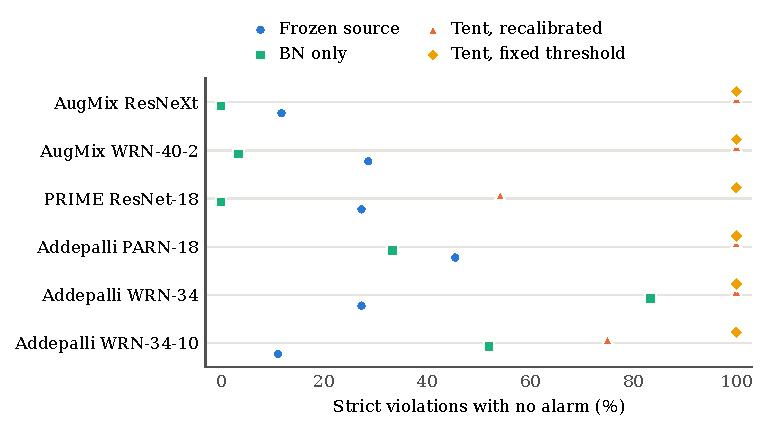
\includegraphics[width=0.85\linewidth]{figures/missed_by_model.pdf}
\caption{Missed share by checkpoint and arm in the factorial study. Counts are in Table~\ref{tab:models}. Arms are distinguished by marker shape as well as color.}
\label{fig:models}
\end{figure}

\subsection{Exploratory: what the monitor can see}
This analysis was written after all verdicts were known and enters no rule. Fig.~\ref{fig:split} splits predictions on strict streams into three parts. Error is similar across arms, but under Tent the flagged rate falls from 0.65 to 0.43, and unflagged errors increase from 0.07 to 0.21. BN's split matches the frozen model's. Within a Tent stream, the flagged rate falls from 0.48 in the first half to 0.39 in the second, while error stays near 0.51. In 87 of Tent's 94 recalibrated misses, the stream-average flagged rate minus $L_1$ did not reach the alarm level, which suggests that a tighter confidence sequence alone would rarely have rescued them. The same held for 16 of BN's 37 misses and 6 of source's 18. This is a stream-average summary and not a population limit. On draws where both arms violated, Tent alone was missed on 77 and BN alone on 1, across 108 draws with a mean error difference of $-0.04$. Tent exceeded BN within the excess-error bands with enough streams: 65/74 against 34/87 at 0.15--0.25, and 27/31 against 3/57 at 0.25--0.35.

\begin{figure}[t]
\centering
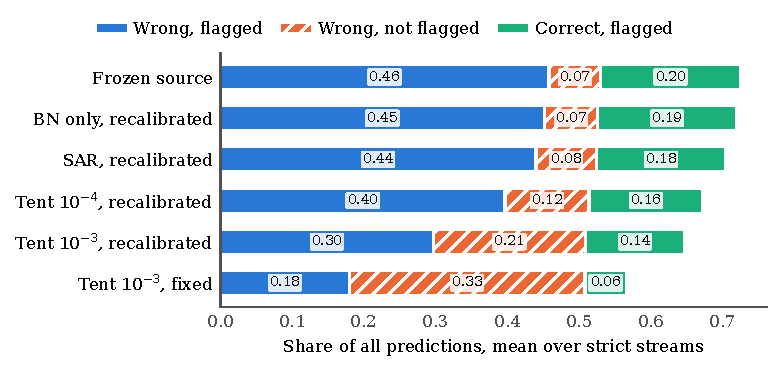
\includegraphics[width=0.85\linewidth]{figures/error_split.pdf}
\caption{Split of predictions on strict streams, as an equal-weight mean over models. Each arm has its own strict set. Error is the sum of the two ``wrong'' parts; the monitor observes only the total flagged share.}
\label{fig:split}
\end{figure}

\subsection{SAR extension}
SAR did not show the gap under the frozen rule: 47 of 159 missed (30\%) against 18 of 73 (25\%) for source, higher in three of six models, with a gap of 0.05. We label this \emph{not shown}. With a fixed threshold it was 51/159, and against BN 47/159 and 37/154. On draws where both violated, SAR alone was missed on 11 and source alone on 14. No SAR stream collapsed, 159 of 192 were strict, and 8 used the numerical fallback.

Exploratory details matter for reading this. Fig.~\ref{fig:split} shows that SAR's split is close to BN's: flagged rate 0.62 and unflagged errors 0.08, at error 0.52. Confidence on its strict streams was 0.36, close to BN's 0.34 and far below Tent's 0.65. This fits the pattern that the blindness appears when errors shift below the threshold, but it does not show that SAR's design removes the problem. SAR's margin kept only 4--9\% of samples on the four low-confidence checkpoints, so on those models it may barely have adapted, and its learning rate is lower than Tent's. SAR's mean error over its streams was also no better than BN's on those four models. On the two AugMix models, where it kept about 70\% of samples, results differ: AugMix ResNeXt rose to 10/26 missed, against 2/17 for source, while AugMix WRN-40-2 stayed at 1/28. Tent with Adam at the lower learning rate of $10^{-4}$ still showed a gap (0.33), so a small learning rate alone is not an obvious explanation, but SAR's optimizer and filtering effects were not separated.

\subsection{Exploratory: error capture and adjusted estimates}
These analyses use saved streams, were written after all verdicts and enter no rule. They reproduce the frozen counts exactly. Table~\ref{tab:recall} separates two quantities on strict streams: \emph{error capture}, the share of errors that are flagged, and \emph{flag precision}, the share of flags that are errors. Tent's capture was lower than source's on all six models in both the replication and the factorial, with mean differences of $-0.26$ and $-0.29$. Its precision changed far less, with mean differences of $-0.03$ and $-0.02$, though it was lower on five of six models. BN matched source on both, and SAR was close to it. So Tent's flags remain about as trustworthy, but far fewer errors raise them. This is more specific than a rise in average confidence. Capture also varies widely between models under Tent, from 0.28 on AugMix ResNeXt to 0.76 on Addepalli PARN-18.

Bootstrap intervals for the missed-share gap are in Table~\ref{tab:adjusted}, resampling corruption types within models and, separately, whole models; six models make the latter coarse. To check that Tent's misses do not simply reflect milder violations, we fit a logistic regression of a miss on arm, excess error and model, with standard errors clustered on model and corruption. The adjusted difference in miss probability stayed large for Tent, and near zero for BN. Odds ratios are large but imprecise because many Tent cells are near 100\% missed, so we report the adjusted differences as the main summary. Among streams that did alarm, Tent's alarms also came later: median batch 69 against 28 in the factorial and 77 against 31 in the replication. Few Tent streams alarmed, and those that did may differ from the rest, so this is descriptive.

\begin{table}[t]
\caption{Error capture and flag precision on strict streams, as equal-weight means over models, with the lowest and highest model values for capture. Exploratory.}
\label{tab:recall}
\centering\footnotesize\setlength{\tabcolsep}{5pt}
\resizebox{\linewidth}{!}{%
\begin{tabular}{@{}llccc@{}}
\toprule
Study & Arm & Error capture & Capture range & Flag precision\\
\midrule
Replication & Source & 0.82 & 0.74--0.91 & 0.72\\
 & Tent, recalibrated & 0.57 & 0.28--0.76 & 0.68\\
\midrule
Factorial & Source & 0.86 & 0.77--0.93 & 0.70\\
 & BN, recalibrated & 0.86 & 0.82--0.89 & 0.70\\
 & SAR, recalibrated & 0.84 & 0.80--0.87 & 0.71\\
 & Tent $10^{-4}$, recalibrated & 0.77 & 0.69--0.84 & 0.71\\
 & Tent $10^{-3}$, recalibrated & 0.57 & 0.28--0.76 & 0.68\\
 & Tent $10^{-3}$, fixed & 0.35 & 0.26--0.43 & 0.75\\
\bottomrule
\end{tabular}}
\end{table}

\begin{table}[t]
\caption{Gap in missed share with 95\% bootstrap intervals, and the adjusted difference in miss probability from a logistic regression on arm, excess error and model. Exploratory.}
\label{tab:adjusted}
\centering\footnotesize\setlength{\tabcolsep}{5pt}
\resizebox{\linewidth}{!}{%
\begin{tabular}{@{}lcccc@{}}
\toprule
Comparison & Gap & Corruptions resampled & Models resampled & Adjusted diff.\\
\midrule
Replication: Tent vs.\ source & 0.49 & 0.37 to 0.59 & 0.32 to 0.63 & 0.46\\
Factorial: Tent vs.\ source & 0.62 & 0.51 to 0.72 & 0.42 to 0.78 & 0.60\\
Factorial: Tent vs.\ BN & 0.62 & 0.52 to 0.72 & 0.35 to 0.85 & 0.59\\
Factorial: BN vs.\ source & $-0.01$ & $-0.13$ to 0.12 & $-0.21$ to 0.25 & 0.01\\
\bottomrule
\end{tabular}}
\end{table}

\subsection{Exploratory: false alarms and signal separation}
A monitor could miss more simply because it alarms less everywhere, so we checked alarms on safe streams, defined as mean error below $r_0+0.10$ without collapse. Definitions were written before these rates were computed, after all verdicts. False alarms were rare and not lower under Tent: 2/46 against 1/81 for source in the factorial, and 3/34 against 0/81 in the replication. These counts are too small to show that Tent's rate is higher. BN (0/8) and SAR (0/7) had too few safe streams to assess.

We then asked whether the alarm level alone explains the misses. Let $M$ be the highest value a stream's lower bound reaches, relative to $r_0$. Table~\ref{tab:separation} gives the AUROC of $M$ for strict against safe streams, and the misses when each model's alarm level is reset, with hindsight, to a 5\% false-alarm rate on its safe streams. Only the three Addepalli models have at least five safe and five strict streams in both arms, so the comparison uses those. The frozen model separates almost perfectly, and most of its misses disappear once the level is reset. Tent's separation is lower, and many misses remain. On these models, part of the loss is therefore in the signal and is not only a conservative alarm level. The resets use labels and only 11--15 safe streams per model, so they measure signal quality and are not a usable alarm. The AugMix and PRIME models, BN and SAR cannot be assessed this way. Tent's separation was somewhat higher with a fixed threshold than with recalibration in the factorial, which we did not investigate further.

\begin{table}[t]
\caption{Separation of strict and safe streams on the three Addepalli models, the only ones with enough streams in both arms. Exploratory; the 5\% level is set with hindsight.}
\label{tab:separation}
\centering\footnotesize\setlength{\tabcolsep}{5pt}
\resizebox{\linewidth}{!}{%
\begin{tabular}{@{}llccc@{}}
\toprule
Study & Arm & Mean AUROC & Missed, released alarm & Missed at 5\% false alarms\\
\midrule
Factorial & Source & 0.995 & 9/31 & 1/31\\
 & Tent, recalibrated & 0.788 & 39/43 & 20/43\\
 & Tent, fixed & 0.851 & 43/43 & 14/43\\
\midrule
Replication & Source & 0.977 & 27/51 & 5/51\\
 & Tent, recalibrated & 0.703 & 62/65 & 55/65\\
\bottomrule
\end{tabular}}
\end{table}

\section{An Entropy-Free Twin Alarm}
\subsection{Design}
The results above suggest that the entropy step distorts the sensor while error changes much less. We therefore keep Tent running and stop reading its own confidence. A \emph{twin} of the same checkpoint uses test-batch normalization and takes no gradient steps. Let $F$ mean the twin flags a sample and $A$ mean the two models predict the same class. If the models agree, Tent is wrong exactly when the twin is wrong, so
\begin{equation}
r_{\mathrm{Tent}} \ge P(F,A) + P(\neg F,\neg A) - \mathrm{FP}_{\mathrm{twin}} - \mathrm{FN}_{\mathrm{twin}},
\end{equation}
where $\mathrm{FP}_{\mathrm{twin}}$ and $\mathrm{FN}_{\mathrm{twin}}$ are the twin's joint false-positive and false-negative probabilities on the stream. This holds because a flagged, agreeing sample where Tent is right is a twin false positive, and an unflagged, disagreeing sample where Tent is right has the twin wrong and unflagged. Tent's confidence plays no part in this inequality. We consider the family $z=P(F,A)+wP(F,\neg A)+cP(\neg F,\neg A)$, with $w\in\{0,0.25,0.5,0.75,1\}$ and $c\in\{0,1\}$, and feed $z$ to the same confidence sequence and alarm level. Those stream quantities need labels, so the correction term uses the twin's clean calibration values, which assumes they do not understate the stream's. This is an assumption about the twin, not a guarantee. Only $w=0$ has the inequality above; larger $w$ is heuristic. The twin's threshold is computed once, so the cost is 100 extra forward images per batch, against 1,000 for per-batch recalibration. We did not compare wall time.

\subsection{Evaluation}
Rules were frozen before any twin stream ran. Noise and blur streams, skewed and balanced, were used to select the candidate with the fewest misses and at most 5\% false alarms. Weather and digital streams, on the same draws as the released monitor, then gave one verdict: the fix works if misses are lower in at least five of six models, the pooled missed share falls by at least 0.40, and false alarms on held-out safe streams, including balanced and clean ones, are at most 10\%. Runs used an H100; same-draw Tent error differed from the RTX 4090 runs by a median of 0.0007.

\subsection{Results}
Selection chose $w=1,c=1$: flag if the twin is uncertain or the models disagree. The frozen verdict was \emph{fix works}: 30/115 missed against 94/109, lower in all six models, a fall of 0.60 (model bootstrap 0.33 to 0.82), with 5/121 false alarms (Table~\ref{tab:twin}). On draws where both versions faced a strict violation, the twin alone missed 1 and the released monitor alone missed 65 of 109. On the same safe skewed streams, false alarms were 3/46 against 2/46. The median first alarm among alarming streams was batch 34, against 69. On the three Addepalli models, AUROC rose from 0.788 to 0.94, and misses at a hindsight 5\% false-alarm level fell from 20/43 to 11/46.

The limits are substantial. The certified forms missed all 115 violations, so the inequality is valid but not useful here. The selected form is a detector, not a bound: its stream-average estimate exceeded Tent's error on 86\% of AugMix ResNeXt streams and 0--26\% on the others. When Tent was safe while the twin was strictly violating, it false-alarmed on 4/13. The Addepalli models remain weak at 29/46 missed, against 1/69 on the other three. In these streams, no Tent violation occurred with the twin below the alarm level, so nearly all failures were shared by the two models.

\begin{table}[t]
\caption{Held-out missed violations per checkpoint. The twin rule was selected on development corruptions. Certified form: $w=0$.}
\label{tab:twin}
\centering\footnotesize\setlength{\tabcolsep}{5pt}
\resizebox{\linewidth}{!}{%
\begin{tabular}{@{}lccc@{}}
\toprule
Checkpoint & Released & Twin alarm ($w=1,c=1$) & Certified\\
\midrule
\texttt{Hendrycks2020AugMix\_ResNeXt} & 20/20 & 0/21 & 21/21\\
\texttt{Hendrycks2020AugMix\_WRN} & 22/22 & 1/23 & 23/23\\
\texttt{Modas2021PRIMEResNet18} & 13/24 & 0/25 & 25/25\\
\texttt{Addepalli2021Towards\_PARN18} & 12/12 & 10/13 & 13/13\\
\texttt{Addepalli2021Towards\_WRN34} & 15/15 & 12/16 & 16/16\\
\texttt{Addepalli2022Efficient\_WRN\_34\_10} & 12/16 & 7/17 & 17/17\\
\midrule
Pooled & 94/109 & 30/115 & 115/115\\
\bottomrule
\end{tabular}}
\end{table}

\subsection{Test on adaptation-caused failures}
Because those streams contained no failure unique to Tent, we froze a second test. Tent ran with Adam at learning rates $10^{-2}$ and $5\times10^{-2}$ on clean and severity-1 streams, with the twin rule unchanged. A target stream has Tent error at least $r_0+0.15$, including collapse, with twin error below $r_0+0.10$. The rule needed at least 75\% detection and at most 10\% false alarms on safe streams.

The twin alarm passed the detection criterion\footnote{The frozen rule combined detection with the false-alarm limit, and its combined outcome was \emph{not shown}, because 1 of 6 safe streams alarmed. This does not make the test a failure of the alarm: the limit had no minimum number of safe streams, a design flaw of ours, and the exact 95\% interval for 1/6 is 0.4\% to 64\%, which neither supports nor rules out a 10\% rate.}: it fired on 51 of 61 target streams (84\%; exact 95\% interval 72\% to 92\%), against 23 of 61 for the released monitor. On the same six safe streams, it alarmed on 1 and the released monitor on 3. We read this test as uninformative on false alarms, not as evidence of a high rate. At the usual learning rate, with far more safe streams, the held-out false-alarm rate was 5/121, with an interval of 1.4\% to 9.4\%, though under different conditions. The detection result is also narrow: 56 of the 61 targets collapsed, and on the 5 that did not, the twin caught 3 and the released monitor 2. The advantage comes from the highest learning rate (34/34 against 3/34). At $10^{-2}$, the released monitor did better (20/27 against 17/27). All 53 balanced targets and 8 Dirichlet targets are included in these counts. On by-class clean streams, the twin's own error also rose 0.40--0.52 above $r_0$, so these are not adaptation-only failures, and both monitors alarmed on all 12. These results should be taken with caution: the twin alarm clearly sees extreme adaptation-caused collapse, while its detection of subtler harm from adaptation and its false-alarm rate in this regime remain open.

\section{Discussion}
\textbf{Interpretation.} A confidence-based sequential monitor can be statistically valid and still be far less sensitive on the adapted model than on its frozen counterpart. Taken together, the results point to Tent's entropy step moving errors below the threshold more than recalibration on clean data can correct. The clean calibration set does not show the corrupted stream's behavior, which is one plausible reason, but we did not test it. We have identified which arm adds the misses, not which change inside the network causes them.

\textbf{Practical implication.} A silent monitor should not be read as a safety signal for a Tent-adapted model under corruption and class skew, and our SAR result does not show that silence is safe under other methods. Validity and detection power should be evaluated separately, and adapted and frozen models should be compared directly when a monitor is evaluated.

\textbf{Limits.} We studied one dataset and one skew construction with replacement sampling. The gap was shown for Tent and not shown for SAR at default settings, so the results must not be generalized to all entropy-based methods, and other methods remain untested. The SAR, twin and adaptation-harm runs used an H100, while the comparison arms used an RTX 4090. The six checkpoints were also those in which the pattern was first noticed, and held-out image IDs had been used in earlier confirmation work. Each arm is conditioned on its own violations, so the comparison populations differ; paired draws and excess-error bands reduce this concern but do not eliminate it. Some streams used a predictable-mixture confidence sequence as a numerical fallback (31 of 768 factorial streams). Authors' pipeline results needed a disclosed loader patch, run-time stream replacement and torch 1.11, and streams that ran out of GPU memory were rerun with fewer processes, with no results replaced. Dirichlet(0.1) is a stress case, and we do not know how common it is in deployment. False-alarm counts are small, and the separation analysis covers three of six models. The twin alarm was not compared with other alternatives, such as the prototype-distance proxy in~\cite{Schirmer2025Monitoring} or independent estimators~\cite{Lee2024AETTA,Garg2022ATC}, and frozen-reference checks already exist in other settings~\cite{Han2026Exchangeability}, so we do not claim it is new in concept. Its test on failures caused by adaptation used deliberately extreme learning rates and had few safe and few non-collapsed streams, so its pass on detection should be read with caution.

\section{Conclusion}
Under strong class skew and corruption on CIFAR-100-C, a released label-free risk monitor missed Tent's clear risk violations far more often than those of the frozen model, in our implementation and in the authors' own code. The gap does not depend on threshold recalibration, and Tent's entropy step adds to it beyond normalization updates. The gap was not shown for SAR at its default settings, where flagged rates and confidence stayed close to normalization alone. An entropy-free twin alarm, tuned on separate corruptions, recovered much of the lost sensitivity at low false-alarm rates on failures shared with the twin, without a certified bound; it also detected most extreme adaptation-caused collapses, though subtler harm and false alarms in that regime remain open. These results extend a known family of proxy failures with a controlled measurement and a practical mitigation. Future work should repeat the adaptation-harm test with a minimum number of safe and non-collapsed streams set in advance, so that false alarms and subtler harm can be measured properly. The other next tests are other datasets and adaptation methods, separating SAR's filtering and optimizer effects, and alternatives compared at matched false-alarm rates.

\bibliographystyle{splncs04}
\bibliography{references}
\end{document}
